\chapter{Allgemeines}

Der \textbf{Backend-Server} hat die Aufgabe, durch den Abruf bestimmter Routes Daten, der Datenbank des Systems zu verändern. Damit dies möglich ist besteht ein Backend-System aus zwei Teilen:

\begin{itemize}
    \item \textbf{Datenbankverbindung}
    \item \textbf{REST-API}
\end{itemize}

Für die Entwicklung des Servers wurde die Programmiersprache Javascript verwendet.

\section{Datenbankverbindung}

Beim Starten der Anwendung wird zu aller erst eine Verbindung zum MySQL Server mit Hilfe der MySQL Libary aufgebaut, welche auf einem Docker-Container läuft. Die Anmeldedaten der Datenbank

liegen in den versteckt in den Docker Secrets.



\section{Konfiguration}

Zur Konfiguration des Backend-Servers werden die Konfigurationswerte zuerst in den Umgebungsvariablen gesucht. Falls keine Werte gefunden werden, wird in den Docker Secrets gesucht.

\label{dockersecrets}

\textbf{Docker Secrets} erlaubt es, sensitive Daten wie Passwörter oder Zugangsschlüssel sicher auf einem Server zu speichern. Im Fall von Sokka werden \lstinline{MYSQL_DB}, \lstinline{MYSQL_HOST}, \lstinline{MYSQL_USERNAME}, \lstinline{MYSQL_PASSWORD}, \lstinline{VERIFY_EMAIL} und \lstinline{VERIFY_EMAIL_PASSWORD} gespeichert.

Die Secrets müssen in Textdateien in einem vom VCS ausgenommenen Ordner erstellt werden. Diese Textdateien müssen anschließend bei der Erstellung der Container, in unserem Fall in der \lstinline{docker-compose.yml}, eingetragen werden. Beim Start der Container werden alle Secrets in die Container an den Pfad \lstinline{/run/secrets/<key>} kopiert, wo sie schlussendlich ausgelesen werden können.

\begin{code}[htp]
    \begin{center}
        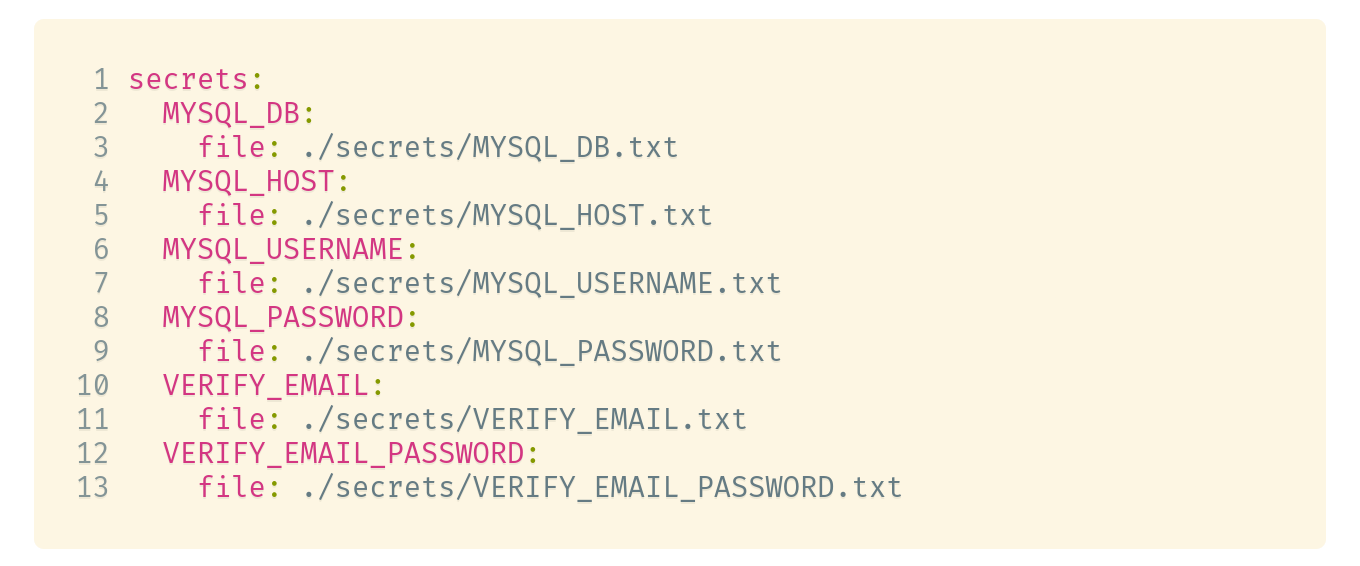
\includegraphics[width=1\textwidth]{images/Backend/secrets.png}
        \vspace{-25pt}
        \caption{Sokkas Docker Secrets in der \lstinline{docker-compose.yml}}
    \end{center}
\end{code}

\section{REST-API}

Damit die App und die Website auf die Daten der Datenbank zugreifen können, stellt der Server sogenannte Rest-Routes zur Verfügung. Jeder Computer mit Internetzugang kann auf diese Routes zugreifen insofern, die Richtigen HTTPs Anfragen an den Server gesendet werden.

Eine vollständige Dokumentation alles Rest-Routes befindet sich im Kapitel Rest-Routes-Dokumentation


\subsection{Bilder}

Bei \textbf{Skate-Buddy} erhalten sowohl die Skateparks, sowohl als auch ihre Obstacle Bilder. Um diese

